% !TeX root = ../main.tex
% Add the above to each chapter to make compiling the PDF easier in some editors.

\chapter{Method}
\section{Communication Compression}
\begin{figure}
\centering
    \begin{subfigure}{.70\textwidth}
        \centering
        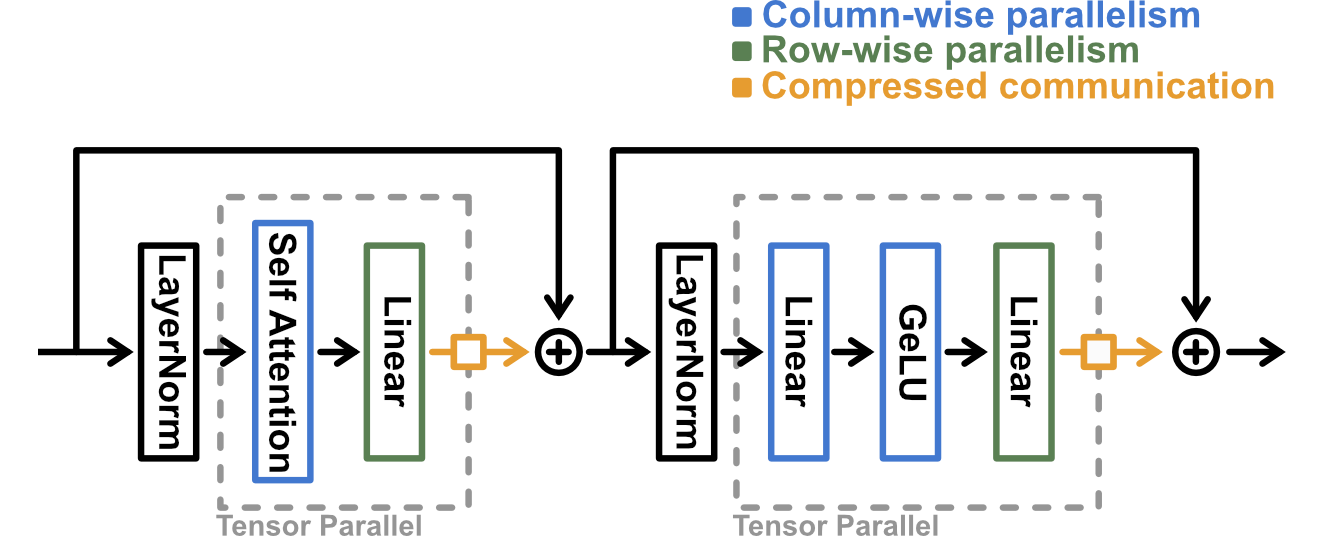
\includegraphics[width=1\linewidth]{figures/overview_arch.png}
        %\caption{An illustration of TP applied to GPT based model, \\ including our activation compression (shown in orange).}
        \caption{}
        \label{fig:overview_arch}
    \end{subfigure} % \hfill

    \begin{subfigure}{.70\textwidth}
        \centering
 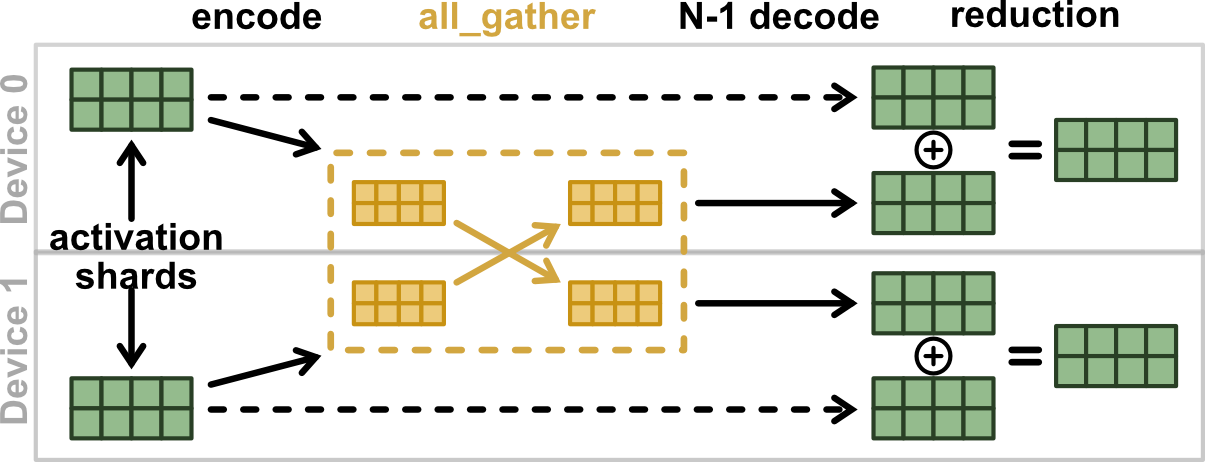
\includegraphics[width=1\linewidth]{figures/overview_comms.png}
        %\caption{An illustration of our approach of compressing the all\_gather collective.}
        \caption{}
        \label{fig:overview_comms}
    \end{subfigure}
\caption{An illustration of transformer-based LLM model parallelized using TP. In Figure \ref{fig:overview_arch}, column-wise and row-wise TP layers are marked blue and red, respectively. Before reduction, we propose to compress the all\_gather collective op (orange in Figure \ref{fig:overview_arch}), as presented in Figure \ref{fig:overview_arch}.}
% Activation shards from the row-wise TP layers are being synchronized using the all\_gather collective op across devices before reduction, which we propose to compress as shown in Figure.}
\label{fig:overview}
\end{figure}

We aim at compressing communication between accelerators, among which a LLM is sharded using tensor-parallelism. As highlighted in Figure (\ref{fig:overview}), linear layers within all attention and MLP blocks are sharded, following common approaches \parencite{megatron, reducingactivationrecomputation}. Distributing layers in this fashion minimizes the number of necessary synchronization operations effectively, making only a single synchronization after each row-wise TP layer necessary. Hence, to compress communication between accelerators, we only need to consider these row-wise TP layers. 

As presented in Figure (\ref{fig:overview_comms}), we achieve this by compressing the partial results of each worker after row-wise TP linear layers, and decompressing them before reduction in each worker. 
To accomplish this in the most effective way, we require compression appraches which...
\begin{enumerate}
    \item compress activations to very low bit widths, e.g. 4 bits
    \item are accurate and can deal with the dynamic nature of activations, since we want to avoid significant model performance degradation
    \item fast compression schemes, since compression and decompression  introduces extra computations which offsets slower inter-accelerator communication
\end{enumerate}
To strike the right balance between these 3 points, which are in general... antiproportional???, we describe in the following our approach of assessing the performance of quantization approaches.

\section{Method Evaluation}
\begin{itemize}
    \item we investigate different quantization approaches
    \item to assess their performance, we divide it into 2 parts: numerical experiments, where we assess their quantization accuracy; and profiling, where we measure the actual TTFT speedups in a deployment scenario
    \item both together are necessary for determining the effectiveness of approaches
    \item we do this split, because
        \begin{itemize}
            \item easier experimentation: we use deepspeed (zero-3) for offloading, enabling us to run larger models with few, small GPUs; aswell simpler experimentation framework
            \item for profiling, running different server setups is important, not necessary for numerical experiments
        \end{itemize}
\end{itemize}

\subsection{Numerical Performance}
We measure the compression rate of compression approaches based on the compression rate, which is measured by the number of \textit{effective bits} \parencite{gptq, awq}. \textcolor{red}{example for group quantization}

To determine the accuracy of compression approaches, we measure the increase in Perplexity metric \parencite{kvquant, atom, llmint8, outliersuppression}, relative to the compression-free model with 16 bit (FP16) activations. Although Perplexity in general isn't very suitable for determining model performance, we deemed it sufficient for our purposes since we are only interested in performance degradation compared to the float model.

We aim at achieving lossless model compression, which is defined by a relative error below 1\% in literature \parencite{mlperf}. \textcolor{red}{do we?? maybe near-lossless... so 1-2\% drop is fine}.

\subsection{Measuring latency improvements}
\begin{itemize}
	\item descripe our hacks? (crop/pad)
\end{itemize}

To show we can reduce communication bottlenecks by utilizing our most performant quantization approaches, we measure the TTFT of models of different sizes in a deployment scenario. We base our profiling on the code provided by \cite{ibmfms} which uses \verb|torch.compile| \parencite{torchcompile} to speed up inference of Llama 2 models by optimizing the computation graph, along with TP. The architecture of the Llama 2 model family is very similar to other state-of-the-art LLMs and therefore provides valuable compression insights. We extended the code to add communication compression. In our profiling setup, each worker in a TP group of $N$ workers compresses output activations of each row-wise linear layer before communication, and decompresses N-1 activations gathered from all other workers. We finally reduce the decompressed activations using \verb|torch.sum| as shown in Figure \ref{fig:overview_comms}.




\subsection{Models}
\begin{itemize}
    \item experiment with different model families -> have different outlier characteristica
    \item different model sizes
    \item some smaller experiments are only conducted with small models for faster experimentation
\end{itemize}
